%%%%%%%% ICML 2025 TEMPLATE USED FOR THIS PAPER %%%%%%%%%%%%%%%%%

\documentclass{article}

\usepackage{microtype}
\usepackage{graphicx}
\usepackage{subfigure}
\usepackage{booktabs} % for professional tables

% hyperref makes hyperlinks in the resulting PDF.
\usepackage{hyperref}


% Attempt to make hyperref and algorithmic work together better:
\newcommand{\theHalgorithm}{\arabic{algorithm}}

% Use the following line to anonymize the paper for peer review:
\usepackage{icml2025}

% For non-anonymized release, use this instead:
%\usepackage[accepted]{icml2025}

% For theorems and such
\usepackage{amsmath}
\usepackage{amssymb}
\usepackage{mathtools}
\usepackage{amsthm}

% if you use cleveref..
\usepackage[capitalize,noabbrev]{cleveref}

%%%%%%%%%%%%%%%%%%%%%%%%%%%%%%%%
% THEOREMS
%%%%%%%%%%%%%%%%%%%%%%%%%%%%%%%%
\theoremstyle{plain}
\newtheorem{theorem}{Theorem}[section]
\newtheorem{proposition}[theorem]{Proposition}
\newtheorem{lemma}[theorem]{Lemma}
\newtheorem{corollary}[theorem]{Corollary}
\theoremstyle{definition}
\newtheorem{definition}[theorem]{Definition}
\newtheorem{assumption}[theorem]{Assumption}
\theoremstyle{remark}
\newtheorem{remark}[theorem]{Remark}

% Todonotes is useful during development; simply uncomment the next line
%    and comment out the line below the next line to turn off comments
%\usepackage[disable,textsize=tiny]{todonotes}
\usepackage[textsize=tiny]{todonotes}


% The \icmltitle you define below is probably too long as a header.
% Therefore, a short form for the running title is supplied here:
\icmltitlerunning{Exploring a Simplified Approach to Randomized Sampling for Logistic Regression}

\begin{document}

\twocolumn[
\icmltitle{Evaluating the Impact of Randomized Sampling on Diverse Prediction Model Training}

% You can specify symbols, otherwise they are numbered in order.
% Ideally, you should not use this facility. Affiliations will be numbered
% in order of appearance and this is the preferred way.
\icmlsetsymbol{equal}{*}

\begin{icmlauthorlist}
\icmlauthor{Luiz Parente}{equal,lp}
\end{icmlauthorlist}

\icmlaffiliation{lp}{School of Electrical and Computer Engineering, Purdue University, IN, USA}
\icmlcorrespondingauthor{Luiz Parente}{lparente@purdue.edu}

% You may provide any keywords that you
% find helpful for describing your paper; these are used to populate
% the "keywords" metadata in the PDF but will not be shown in the document
\icmlkeywords{Machine Learning, Sampling Algorithm, Leverage Scores}

\vskip 0.3in
]

% this must go after the closing bracket ] following \twocolumn[ ...

% This command actually creates the footnote in the first column
% listing the affiliations and the copyright notice.
% The command takes one argument, which is text to display at the start of the footnote.
% The \icmlEqualContribution command is standard text for equal contribution.
% Remove it (just {}) if you do not need this facility.

%\printAffiliationsAndNotice{}  % leave blank if no need to mention equal contribution
\printAffiliationsAndNotice{\icmlEqualContribution} % otherwise use the standard text.

\begin{abstract}
TBD.
\end{abstract}

\section{Literature Review}
\label{submission}

\subsection{Background}

Test Submission to ICML 2025 will be entirely electronic, via a web site
(not email). Information about the submission process and \LaTeX\ templates
are available on the conference web site at:
\begin{center}
\textbf{\texttt{http://icml.cc/}}
\end{center}

The guidelines below will be enforced for initial submissions and
camera-ready copies. Here is a brief summary:


\subsection{Problem Definition}

\begin{itemize}
\item Submissions must be in PDF\@. 
\item If your paper has appendices, submit the appendix together with the main body and the references \textbf{as a single file}. Reviewers will not look for appendices as a separate PDF file. So if you submit such an extra file, reviewers will very likely miss it.
\item Page limit: The main body of the paper has to be fitted to 8 pages, excluding references and appendices; the space for the latter two is not limited in pages, but the total file size may not exceed 10MB. For the final version of the paper, authors can add one extra page to the main body.
\item \textbf{Do not include author information or acknowledgements} in your
    initial submission.
\item Your paper should be in \textbf{10 point Times font}.
\item Make sure your PDF file only uses Type-1 fonts.
\item Place figure captions \emph{under} the figure (and omit titles from inside
    the graphic file itself). Place table captions \emph{over} the table.
\item References must include page numbers whenever possible and be as complete
    as possible. Place multiple citations in chronological order.
\item Do not alter the style template; in particular, do not compress the paper
    format by reducing the vertical spaces.
\item Keep your abstract brief and self-contained, one paragraph and roughly
    4--6 sentences. Gross violations will require correction at the
    camera-ready phase. The title should have content words capitalized.
\end{itemize}

\subsection{Summary and Critique of the Selected Papers}


\subsubsection{Main Paper: A Provably Accurate Randomized Sampling Algorithm for Logistic Regression \cite{chow24}}

\textbf{Summary:} Logistic regression is a widely used method for binary classification tasks, where the goal is to predict one of two possible outcomes based on input features \cite{pml}. However, when the number of observations greatly exceeds the number of predictor variables, solving logistic regression becomes computationally expensive. In this work, \citeauthor{chow24} propose a novel approach to address this issue by leveraging a randomized sampling technique that guarantees high-quality approximations to the estimated probabilities of logistic regression, with a sample size significantly smaller than the total number of observations. The primary goal is to make logistic regression more computationally efficient for large-scale datasets while maintaining prediction accuracy.

The paper focuses on the use of leverage scores, which is a method that, given a dataset, allows for the extraction of a subset where the derived data points retain the main characteristics of the overall data \cite{ordo22}. The authors' proposed algorithm constructs a sampling matrix using these scores, and the resulting subsampled log-likelihood function is optimized to estimate the model parameters. This randomized approach allows for substantial reductions in computational cost while preserving the accuracy of the regression model.
The paper provides a theoretical derivation of an approximation bound that guarantees the accuracy of the estimated probabilities obtained from the subsampled data. This result is significant because it shows that only a small subset of the data may be needed to achieve a high-quality approximation of the original data, making the algorithm more scalable and efficient.

To validate their approach, the authors conduct extensive empirical evaluations on real-world datasets, including a cardiovascular disease prediction dataset, a customer churn prediction dataset, and a credit card default prediction dataset. The experiments compare the performance of the proposed leverage score-based sampling method with other sampling schemes, including uniform sampling and the L2S method proposed by \citeauthor{mun18}. The results demonstrate that the leverage score-based method performs comparably to other methods in terms of the accuracy of estimated probabilities, and shows potential for outperformance, particularly as the sample size increases. Moreover, the method achieves misclassification rates close to those obtained by the full-data model, further confirming its effectiveness. These empirical results validate the theoretical claims and show that the proposed algorithm can deliver accurate logistic regression estimates with a reduced sample size.

The paper concludes with a discussion about the implications of their findings and suggesting future research directions. While the proposed method performs well in practice, the authors highlight that there is still room for improvement in terms of algorithmic efficiency and scalability, particularly in high-dimensional settings. They also suggest exploring alternative sketching techniques, such as random projection-based methods, to further enhance the sampling process. Additionally, the paper points out that the approach could be extended to handle other forms of regression and machine learning models, making it a valuable tool for a variety of applications. The paper makes a significant contribution by providing an efficient and scalable solution to logistic regression for large datasets, with strong theoretical guarantees and solid empirical results.



\textbf{Critique:} While the paper provides an excellent approach for logistic regression, it does not explore the application of the same sampling algorithm to other types of prediction models. The authors focus exclusively on logistic regression, which is understandable given the complexity and computational challenges associated with large datasets in this context. However, the question of whether the method could potentially be adapted for use with other models, such as linear regression, support vector machines, or even more complex deep learning models, remain unclear. Given that dataset distillation has been an area of interest in machine learning \cite{liu23}, a discussion of how their technique could be generalized or modified for broader applications range would have added valuable insight to the work. Exploring the adaptability of the sampling strategy to a range of prediction models could increase the impact and versatility of the proposed method, making it applicable to a wider array of real-world problems.

Additionally, even though the paper does provide a robust theoretical foundation for the proposed method, it could benefit from a more detailed exploration of the trade-offs between simplicity and accuracy, particularly when it comes to the complexity of the algorithm. While the proposed algorithm is presented as computationally efficient, the authors do not thoroughly investigate alternative variations of the algorithm that might provide different levels of complexity or accuracy. For example, they focus heavily on the use of row leverage scores to select data points, but it would be valuable to see whether simpler strategies could yield comparable performance. Moreover, a discussion of whether implementing theoretical guarantees—such as the approximation bounds—justifies the added complexity would provide a clearer understanding of the practical trade-offs involved. The paper does an excellent job of presenting an efficient solution, but more emphasis on evaluating the balance between theoretical rigor and real-world applicability could enrich the findings.

Another area where the paper could expand is in providing a more nuanced analysis of the error bounds and their impact on the overall model performance. While the theoretical guarantees are a key strength of the paper, there is limited exploration of how these bounds manifest in practice when applied to different types of datasets. It would have been helpful for the authors to conduct experiments that show how varying the sample size and error tolerance affects both the accuracy of the model and the computational efficiency. In addition, the relationship between the size of the dataset, the model's complexity, and the effectiveness of the approximation would have benefited from further elaboration. For example, is there a point at which the error bounds no longer provide substantial improvements, or do they continue to yield significant benefits with increasing complexity? Addressing these questions could further clarify when and why this sampling-based approach is most beneficial, providing a more comprehensive evaluation of its utility in real-world applications.


\subsubsection{Supplementary Paper: SLOE: A Faster Method for Statistical Inference in High-Dimensional
Logistic Regression \cite{yad21}}

\textbf{Summary:} In high-dimensional problems, where the number of features is comparable to or exceeds the number of samples, traditional logistic regression methods, specifically maximum likelihood estimation (MLE), commonly present poor performance. The existing large-sample asymptotic theory for logistic regression approximations fails in these scenarios, leading to inadequate parameter estimates and unreliable statistical inference.

\citeauthor{yad21} propose a novel solution, the Signal Strength Leave-One-Out Estimator (SLOE), to efficiently estimate the signal strength parameter, which is crucial for performing dimensionality corrections. This method significantly improves the practical application of the corrections developed in previous works, making it computationally feasible and faster to implement in real-world applications.

At the core of this paper is the challenge of estimating the signal strength, which is used in dimensionality corrections to adjust the bias and variance in high-dimensional \textbf{logistic regression}. Previous methods, such as the ProbeFrontier heuristic \cite{sur19}, attempted to estimate this signal strength but were computationally expensive and conceptually complex. The proposed SLOE method reparameterizes the problem in terms of a more easily estimated "corrupted" signal strength, which accounts for the noise in the parameter estimates due to finite sample sizes. The paper demonstrates that using this reparameterization, the bias and variance adjustments for MLE can be performed accurately, even in finite samples, which is a significant improvement over traditional methods that rely on large-sample approximations.

One of the key advantages of SLOE is its computational efficiency. While previous heuristics like ProbeFrontier required multiple subsampling iterations and linear programming to estimate the signal strength, SLOE uses a simple and fast approach by leveraging leave-one-out (LOO) techniques. The method estimates the corrupted signal strength using a rank-one update formula that avoids refitting the model multiple times. The paper shows that SLOE achieves a substantial reduction in computation time compared to ProbeFrontier, making it a practical tool for routine use in high-dimensional logistic regression. This efficiency gain is particularly important when working with large datasets, where computational speed is crucial.

The authors provide a detailed theoretical analysis of the SLOE method, showing that it consistently estimates the corrupted signal strength, which is asymptotically equivalent to the true signal strength. The theoretical guarantees underpin the practical reliability of SLOE in high-dimensional settings. Through extensive simulations, the paper illustrates how SLOE improves the accuracy of confidence intervals (CIs) and p-values in logistic regression models. In particular, the corrected CIs generated by SLOE are shown to provide reliable coverage, even in high-dimensional settings where traditional large-sample approximations fail. This is especially important for making sound statistical inferences in fields like genomics and clinical applications, where reliable uncertainty quantification is critical.

This paper ultimately makes an important contribution to the field of high-dimensional statistical inference. The SLOE method introduced by the authors provide a simpler, faster, and more accurate approach to estimating signal strength in high-dimensional logistic regression. SLOE offers a practical solution to the problems caused by large-dimensional data, enabling more reliable statistical inference in these settings. The method is tested and validated on several real-world datasets, including applications to heart disease prediction and genomics, where it outperforms traditional methods in terms of both computational efficiency and statistical accuracy. SLOE paves the way for more robust and computationally feasible dimensionality corrections, making it a valuable tool for applied data science and statistical modeling.

\textbf{Critique:} While the paper addresses the high-dimensional logistic regression setting under the assumption of Gaussian or sub-Gaussian features, it could have further explored how SLOE performs when the data distribution deviates from these assumptions. Many real-world datasets, for example those encountered in genomics, healthcare, or social sciences, often exhibit non-Gaussian characteristics. The authors briefly mention that SLOE works well in the presence of sub-Gaussian features, but a more thorough analysis of how the method generalizes to different data distributions would provide a clearer picture of it performs in diverse settings. A discussion on this would also be helpful in understanding whether additional steps are needed when dealing with non-Gaussian data, making the method even more applicable across different domains.

In addition, since the paper focuses on overcoming challenges in high-dimensional logistic regression, it could have offered a more detailed comparison to other dimensionality reduction techniques commonly used in similar settings, such as principal component analysis (PCA), partial least squares (PLS), or feature selection methods. These methods are often used in high-dimensional regression problems to reduce the number of predictors, making it more manageable to estimate models. A brief discussion on how SLOE compares or complements these dimensionality reduction techniques would provide additional insights on when to use SLOE versus other popular methods, and whether it offers specific advantages or disadvantages depending on the type of dataset or the modeling goal.

Lastly, one area that could have been explored in more depth is the scalability of the SLOE method to extremely large datasets. The computational efficiency of SLOE is emphasized, particularly in comparison to ProbeFrontier, but the paper could have provided more concrete examples or benchmarks when the dataset size approaches millions of samples, which can be of particular interest in modern real-world applications driven by big data. While the authors demonstrate that SLOE is much faster than its competitors, additional discussion around its performance in ultra-large datasets would be valuable, as it would allow the paper to transcend the academic domain and make a connection with common industry challenges.

\subsubsection{Supplementary Paper: Stable learning via sample reweighting \cite{shen20}}

The paper aims to address the problem of model instability in machine learning, especially when there is a mismatch between training and test data distributions. In real-world scenarios, it is often unrealistic to assume that the training data and the test data come from the same distribution. This discrepancy can lead to unreliable performance, especially when the model relies heavily on collinear input variables. \citeauthor{shen20} aim to develop a method that ensures stability in predictions, even when the underlying data distribution changes. Their work is focused on linear models, which are commonly used for regression and classification tasks but are sensitive to collinearity, which can significantly distort parameter estimates and lead to unstable predictions.

A central challenge addressed in this paper is the impact of collinearity on model stability. Collinearity occurs when there is a high correlation between input variables, leading to a sub-optimal design matrix. This problem is particularly notable in high-dimensional settings, where variables are highly interdependent. The authors argue that traditional methods, such as ordinary least squares (OLS), are susceptible to this issue, causing large errors in parameter estimation when the training data differs from the test data. In particular, they show that even small model misspecifications can lead to large errors in predictions due to the instability introduced by collinearity. Thus, the paper emphasizes the need for a robust approach that can mitigate the adverse effects of collinearity.

To address this issue, the authors propose a novel method called Sample Reweighted Decorrelation Operator (SRDO). This method works by assigning appropriate weights to samples, effectively reweighting the data to reduce collinearity among input variables. By doing so, the design matrix becomes closer to an orthogonal structure, which is more stable and less prone to errors caused by multicollinearity. The theoretical foundation of SRDO shows that, under ideal conditions, the sample weights can make the design matrix nearly orthogonal, significantly improving the model's stability. The method is presented as a general pretreatment technique, meaning it can be integrated with standard linear regression methods like ordinary least squares (OLS), Lasso, and \textbf{logistic regression} to enhance their robustness against distribution shifts.

The paper provides a detailed theoretical analysis of the SRDO method. It demonstrates that, in an idealized setting with infinite sample size, the optimal sample weights can minimize the effects of model misspecification and collinearity. However, the authors also acknowledge the practical challenges when working with finite sample sizes. In such cases, there is a tradeoff between reducing bias and increasing variance, which is common in statistical methods. Despite this, the SRDO method shows a clear advantage in terms of prediction stability and accuracy, especially when the training and test distributions differ significantly. The theoretical results are supported by empirical experiments, which show that SRDO outperforms traditional methods in both regression and classification tasks.

Finally, the paper presents extensive experiments to validate the effectiveness of SRDO. The experiments are conducted using both synthetic and real-world datasets, demonstrating the method's ability to handle collinearity and distribution shifts. The results show that SRDO consistently reduces estimation errors and improves prediction accuracy, especially when training and test data distributions are mismatched. For instance, in the context of regression, SRDO significantly outperforms OLS and Lasso, especially in situations with strong collinearity. In classification tasks, the method also demonstrates improved stability when tested on diverse groups of users with varying behaviors. These findings highlight the practical applicability of SRDO in real-world machine learning scenarios, where data distributions are often subject to change. The authors conclude by emphasizing that SRDO is a versatile and valuable tool for improving the stability and reliability of linear models.

\textbf{Critique:} One area that could have been further explored in the paper is the practical application and limitations of SRDO in real-world datasets with varying feature types. While the authors demonstrate the method’s effectiveness in handling collinearity and improving stability, the paper focuses primarily on linear models, which might not capture more complex patterns in the data. The authors could have discussed how SRDO performs when applied to datasets that involve both linear and non-linear relationships or datasets with categorical features. This would help extend the method’s applicability and provide guidance for researchers working in diverse domains, especially those dealing with non-linear or high-dimensional data. A more in-depth exploration of SRDO’s limitations in such contexts would be beneficial for understanding where the method might fall short or require adaptations.

Furthermore, the authors could have more thoroughly explored the computational complexity and scalability of the proposed method. Despite the strong focus on the theoretical benefits and empirical performance of SRDO, there is little discussion on the practical aspects of implementing the method at scale. The process of calculating and applying sample weights, especially for large datasets with high-dimensional feature spaces, could be computationally expensive. This challenge is particularly important for real-world applications where datasets can contain millions of samples and variables. An analysis of the time complexity of the method, along with potential optimizations or approximations, could provide valuable insights when applying SRDO in large-scale problems.

Another aspect that could have been addressed more thoroughly is the relationship between SRDO and existing regularization techniques for handling collinearity, such as Ridge or Lasso regression. While the paper emphasizes the novel approach of reweighting samples to reduce collinearity, it would have been useful to see a direct comparison with these established methods to better understand whether there are scenarios in which one method presents advantages relative to the others.


\section{Implementation}

All submissions must follow the specified format.


\subsection{Preliminary Setup}

The text of the paper should be formatted in two columns, with an
overall width of 6.75~inches, height of 9.0~inches, and 0.25~inches
between the columns. The left margin should be 0.75~inches and the top
margin 1.0~inch (2.54~cm). The right and bottom margins will depend on
whether you print on US letter or A4 paper, but all final versions
must be produced for US letter size.
Do not write anything on the margins.

The paper body should be set in 10~point type with a vertical spacing
of 11~points. Please use Times typeface throughout the text.

\subsection{Preliminary Implementation Effort}

The paper title should be set in 14~point bold type and centered
between two horizontal rules that are 1~point thick, with 1.0~inch
between the top rule and the top edge of the page. Capitalize the
first letter of content words and put the rest of the title in lower
case.

\subsection{Challenges}

ICML uses double-blind review, so author information must not appear. If
you are using \LaTeX\/ and the \texttt{icml2025.sty} file, use
\verb+\icmlauthor{...}+ to specify authors and \verb+\icmlaffiliation{...}+ to specify affiliations. (Read the TeX code used to produce this document for an example usage.) The author information
will not be printed unless \texttt{accepted} is passed as an argument to the
style file.
Submissions that include the author information will not
be reviewed.

\subsubsection{Self-Citations}

If you are citing published papers for which you are an author, refer
to yourself in the third person. In particular, do not use phrases
that reveal your identity (e.g., ``in previous work \cite{chow24}, we
have shown \ldots'').

Do not anonymize citations in the reference section. The only exception are manuscripts that are
not yet published (e.g., under submission). If you choose to refer to
such unpublished manuscripts \cite{anonymous}, anonymized copies have
to be submitted
as Supplementary Material via OpenReview\@. However, keep in mind that an ICML
paper should be self contained and should contain sufficient detail
for the reviewers to evaluate the work. In particular, reviewers are
not required to look at the Supplementary Material when writing their
review (they are not required to look at more than the first $8$ pages of the submitted document).

\subsubsection{Camera-Ready Author Information}
\label{final author}

If a paper is accepted, a final camera-ready copy must be prepared.
%
For camera-ready papers, author information should start 0.3~inches below the
bottom rule surrounding the title. The authors' names should appear in 10~point
bold type, in a row, separated by white space, and centered. Author names should
not be broken across lines. Unbolded superscripted numbers, starting 1, should
be used to refer to affiliations.

Affiliations should be numbered in the order of appearance. A single footnote
block of text should be used to list all the affiliations. (Academic
affiliations should list Department, University, City, State/Region, Country.
Similarly for industrial affiliations.)

Each distinct affiliations should be listed once. If an author has multiple
affiliations, multiple superscripts should be placed after the name, separated
by thin spaces. If the authors would like to highlight equal contribution by
multiple first authors, those authors should have an asterisk placed after their
name in superscript, and the term ``\textsuperscript{*}Equal contribution"
should be placed in the footnote block ahead of the list of affiliations. A
list of corresponding authors and their emails (in the format Full Name
\textless{}email@domain.com\textgreater{}) can follow the list of affiliations.
Ideally only one or two names should be listed.

A sample file with author names is included in the ICML2025 style file
package. Turn on the \texttt{[accepted]} option to the stylefile to
see the names rendered. All of the guidelines above are implemented
by the \LaTeX\ style file.

\subsection{Next Steps}

The paper abstract should begin in the left column, 0.4~inches below the final
address. The heading `Abstract' should be centered, bold, and in 11~point type.
The abstract body should use 10~point type, with a vertical spacing of
11~points, and should be indented 0.25~inches more than normal on left-hand and
right-hand margins. Insert 0.4~inches of blank space after the body. Keep your
abstract brief and self-contained, limiting it to one paragraph and roughly 4--6
sentences. Gross violations will require correction at the camera-ready phase.


\subsection{Proposal for Course Project}

\subsubsection{Methodology}

You should organize your paper into sections and paragraphs to help
readers place a structure on the material and understand its
contributions.

\subsubsection{Feasibility}

Section headings should be numbered, flush left, and set in 11~pt bold
type with the content words capitalized. Leave 0.25~inches of space
before the heading and 0.15~inches after the heading.

Similarly, subsection headings should be numbered, flush left, and set
in 10~pt bold type with the content words capitalized. Leave
0.2~inches of space before the heading and 0.13~inches afterward.

Finally, subsubsection headings should be numbered, flush left, and
set in 10~pt small caps with the content words capitalized. Leave
0.18~inches of space before the heading and 0.1~inches after the
heading.

Please use no more than three levels of headings.

\subsubsection{Relevance}

Within each section or subsection, you should further partition the
paper into paragraphs. Do not indent the first line of a given
paragraph, but insert a blank line between succeeding ones.

You can use footnotes\footnote{Footnotes
should be complete sentences.} to provide readers with additional
information about a topic without interrupting the flow of the paper.
Indicate footnotes with a number in the text where the point is most
relevant. Place the footnote in 9~point type at the bottom of the
column in which it appears. Precede the first footnote in a column
with a horizontal rule of 0.8~inches.\footnote{Multiple footnotes can
appear in each column, in the same order as they appear in the text,
but spread them across columns and pages if possible.}

\begin{figure}[ht]
\vskip 0.2in
\begin{center}
\centerline{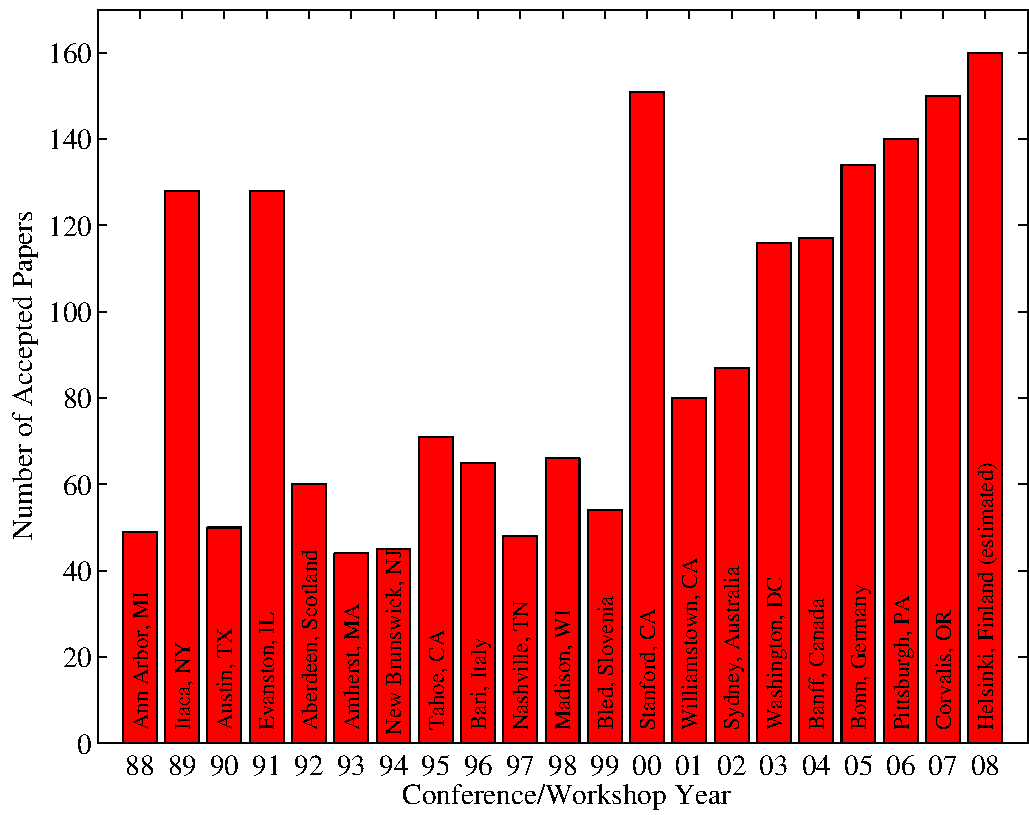
\includegraphics[width=\columnwidth]{icml_numpapers}}
\caption{Historical locations and number of accepted papers for International
Machine Learning Conferences (ICML 1993 -- ICML 2008) and International
Workshops on Machine Learning (ML 1988 -- ML 1992). At the time this figure was
produced, the number of accepted papers for ICML 2008 was unknown and instead
estimated.}
\label{icml-historical}
\end{center}
\vskip -0.2in
\end{figure}

\section{Conclusion}

You may want to include figures in the paper to illustrate
your approach and results. Such artwork should be centered,
legible, and separated from the text. Lines should be dark and at
least 0.5~points thick for purposes of reproduction, and text should
not appear on a gray background.

Label all distinct components of each figure. If the figure takes the
form of a graph, then give a name for each axis and include a legend
that briefly describes each curve. Do not include a title inside the
figure; instead, the caption should serve this function.

Number figures sequentially, placing the figure number and caption
\emph{after} the graphics, with at least 0.1~inches of space before
the caption and 0.1~inches after it, as in
\cref{icml-historical}. The figure caption should be set in
9~point type and centered unless it runs two or more lines, in which
case it should be flush left. You may float figures to the top or
bottom of a column, and you may set wide figures across both columns
(use the environment \texttt{figure*} in \LaTeX). Always place
two-column figures at the top or bottom of the page.

\subsection{Algorithms}

If you are using \LaTeX, please use the ``algorithm'' and ``algorithmic''
environments to format pseudocode. These require
the corresponding stylefiles, algorithm.sty and
algorithmic.sty, which are supplied with this package.
\cref{alg:example} shows an example.

\begin{algorithm}[tb]
   \caption{Bubble Sort}
   \label{alg:example}
\begin{algorithmic}
   \STATE {\bfseries Input:} data $x_i$, size $m$
   \REPEAT
   \STATE Initialize $noChange = true$.
   \FOR{$i=1$ {\bfseries to} $m-1$}
   \IF{$x_i > x_{i+1}$}
   \STATE Swap $x_i$ and $x_{i+1}$
   \STATE $noChange = false$
   \ENDIF
   \ENDFOR
   \UNTIL{$noChange$ is $true$}
\end{algorithmic}
\end{algorithm}

\subsection{Tables}

You may also want to include tables that summarize material. Like
figures, these should be centered, legible, and numbered consecutively.
However, place the title \emph{above} the table with at least
0.1~inches of space before the title and the same after it, as in
\cref{sample-table}. The table title should be set in 9~point
type and centered unless it runs two or more lines, in which case it
should be flush left.

% Note use of \abovespace and \belowspace to get reasonable spacing
% above and below tabular lines.

\begin{table}[t]
\caption{Classification accuracies for naive Bayes and flexible
Bayes on various data sets.}
\label{sample-table}
\vskip 0.15in
\begin{center}
\begin{small}
\begin{sc}
\begin{tabular}{lcccr}
\toprule
Data set & Naive & Flexible & Better? \\
\midrule
Breast    & 95.9$\pm$ 0.2& 96.7$\pm$ 0.2& $\surd$ \\
Cleveland & 83.3$\pm$ 0.6& 80.0$\pm$ 0.6& $\times$\\
Glass2    & 61.9$\pm$ 1.4& 83.8$\pm$ 0.7& $\surd$ \\
Credit    & 74.8$\pm$ 0.5& 78.3$\pm$ 0.6&         \\
Horse     & 73.3$\pm$ 0.9& 69.7$\pm$ 1.0& $\times$\\
Meta      & 67.1$\pm$ 0.6& 76.5$\pm$ 0.5& $\surd$ \\
Pima      & 75.1$\pm$ 0.6& 73.9$\pm$ 0.5&         \\
Vehicle   & 44.9$\pm$ 0.6& 61.5$\pm$ 0.4& $\surd$ \\
\bottomrule
\end{tabular}
\end{sc}
\end{small}
\end{center}
\vskip -0.1in
\end{table}

Tables contain textual material, whereas figures contain graphical material.
Specify the contents of each row and column in the table's topmost
row. Again, you may float tables to a column's top or bottom, and set
wide tables across both columns. Place two-column tables at the
top or bottom of the page.

\subsection{Theorems and such}
The preferred way is to number definitions, propositions, lemmas, etc. consecutively, within sections, as shown below.
\begin{definition}
\label{def:inj}
A function $f:X \to Y$ is injective if for any $x,y\in X$ different, $f(x)\ne f(y)$.
\end{definition}
Using \cref{def:inj} we immediate get the following result:
\begin{proposition}
If $f$ is injective mapping a set $X$ to another set $Y$, 
the cardinality of $Y$ is at least as large as that of $X$
\end{proposition}
\begin{proof} 
Left as an exercise to the reader. 
\end{proof}
\cref{lem:usefullemma} stated next will prove to be useful.
\begin{lemma}
\label{lem:usefullemma}
For any $f:X \to Y$ and $g:Y\to Z$ injective functions, $f \circ g$ is injective.
\end{lemma}
\begin{theorem}
\label{thm:bigtheorem}
If $f:X\to Y$ is bijective, the cardinality of $X$ and $Y$ are the same.
\end{theorem}
An easy corollary of \cref{thm:bigtheorem} is the following:
\begin{corollary}
If $f:X\to Y$ is bijective, 
the cardinality of $X$ is at least as large as that of $Y$.
\end{corollary}
\begin{assumption}
The set $X$ is finite.
\label{ass:xfinite}
\end{assumption}
\begin{remark}
According to some, it is only the finite case (cf. \cref{ass:xfinite}) that is interesting.
\end{remark}
%restatable

\subsection{Citations and References}

Please use APA reference format regardless of your formatter
or word processor. If you rely on the \LaTeX\/ bibliographic
facility, use \texttt{natbib.sty} and \texttt{icml2025.bst}
included in the style-file package to obtain this format.

Citations within the text should include the authors' last names and
year. If the authors' names are included in the sentence, place only
the year in parentheses, for example when referencing Arthur Samuel's
pioneering work \yrcite{Samuel59}. Otherwise place the entire
reference in parentheses with the authors and year separated by a
comma \cite{Samuel59}. List multiple references separated by
semicolons \cite{shen20,Samuel59,yad21}. Use the `et~al.'
construct only for citations with three or more authors or after
listing all authors to a publication in an earlier reference \cite{MachineLearningI}.

Authors should cite their own work in the third person
in the initial version of their paper submitted for blind review.
Please refer to \cref{author info} for detailed instructions on how to
cite your own papers.

Use an unnumbered first-level section heading for the references, and use a
hanging indent style, with the first line of the reference flush against the
left margin and subsequent lines indented by 10 points. The references at the
end of this document give examples for journal articles \cite{Samuel59},
conference publications \cite{chow24}, book chapters \cite{Newell81}, books
\cite{DudaHart2nd}, edited volumes \cite{MachineLearningI}, technical reports
\cite{yad21}, and dissertations \cite{shen20}.

Alphabetize references by the surnames of the first authors, with
single author entries preceding multiple author entries. Order
references for the same authors by year of publication, with the
earliest first. Make sure that each reference includes all relevant
information (e.g., page numbers).

Please put some effort into making references complete, presentable, and
consistent, e.g. use the actual current name of authors.
If using bibtex, please protect capital letters of names and
abbreviations in titles, for example, use \{B\}ayesian or \{L\}ipschitz
in your .bib file.

\section*{Accessibility}
Authors are kindly asked to make their submissions as accessible as possible for everyone including people with disabilities and sensory or neurological differences.
Tips of how to achieve this and what to pay attention to will be provided on the conference website \url{http://icml.cc/}.

\section*{Software and Data}

If a paper is accepted, we strongly encourage the publication of software and data with the
camera-ready version of the paper whenever appropriate. This can be
done by including a URL in the camera-ready copy. However, \textbf{do not}
include URLs that reveal your institution or identity in your
submission for review. Instead, provide an anonymous URL or upload
the material as ``Supplementary Material'' into the OpenReview reviewing
system. Note that reviewers are not required to look at this material
when writing their review.

% Acknowledgements should only appear in the accepted version.
\section*{Acknowledgements}

\textbf{Do not} include acknowledgements in the initial version of
the paper submitted for blind review.

If a paper is accepted, the final camera-ready version can (and
usually should) include acknowledgements.  Such acknowledgements
should be placed at the end of the section, in an unnumbered section
that does not count towards the paper page limit. Typically, this will 
include thanks to reviewers who gave useful comments, to colleagues 
who contributed to the ideas, and to funding agencies and corporate 
sponsors that provided financial support.

\section*{Impact Statement}

Authors are \textbf{required} to include a statement of the potential 
broader impact of their work, including its ethical aspects and future 
societal consequences. This statement should be in an unnumbered 
section at the end of the paper (co-located with Acknowledgements -- 
the two may appear in either order, but both must be before References), 
and does not count toward the paper page limit. In many cases, where 
the ethical impacts and expected societal implications are those that 
are well established when advancing the field of Machine Learning, 
substantial discussion is not required, and a simple statement such 
as the following will suffice:

``This paper presents work whose goal is to advance the field of 
Machine Learning. There are many potential societal consequences 
of our work, none which we feel must be specifically highlighted here.''

The above statement can be used verbatim in such cases, but we 
encourage authors to think about whether there is content which does 
warrant further discussion, as this statement will be apparent if the 
paper is later flagged for ethics review.


% In the unusual situation where you want a paper to appear in the
% references without citing it in the main text, use \nocite
%\nocite{chow24}

\bibliography{paper_references}
\bibliographystyle{icml2025}


%%%%%%%%%%%%%%%%%%%%%%%%%%%%%%%%%%%%%%%%%%%%%%%%%%%%%%%%%%%%%%%%%%%%%%%%%%%%%%%
%%%%%%%%%%%%%%%%%%%%%%%%%%%%%%%%%%%%%%%%%%%%%%%%%%%%%%%%%%%%%%%%%%%%%%%%%%%%%%%
% APPENDIX
%%%%%%%%%%%%%%%%%%%%%%%%%%%%%%%%%%%%%%%%%%%%%%%%%%%%%%%%%%%%%%%%%%%%%%%%%%%%%%%
%%%%%%%%%%%%%%%%%%%%%%%%%%%%%%%%%%%%%%%%%%%%%%%%%%%%%%%%%%%%%%%%%%%%%%%%%%%%%%%
\newpage
\appendix
\onecolumn
\section{You \emph{can} have an appendix here.}

You can have as much text here as you want. The main body must be at most $8$ pages long.
For the final version, one more page can be added.
If you want, you can use an appendix like this one.  

The $\mathtt{\backslash onecolumn}$ command above can be kept in place if you prefer a one-column appendix, or can be removed if you prefer a two-column appendix.  Apart from this possible change, the style (font size, spacing, margins, page numbering, etc.) should be kept the same as the main body.
%%%%%%%%%%%%%%%%%%%%%%%%%%%%%%%%%%%%%%%%%%%%%%%%%%%%%%%%%%%%%%%%%%%%%%%%%%%%%%%
%%%%%%%%%%%%%%%%%%%%%%%%%%%%%%%%%%%%%%%%%%%%%%%%%%%%%%%%%%%%%%%%%%%%%%%%%%%%%%%


\end{document}
